\setlength{\baselineskip}{20pt}
\setlength{\tabcolsep}{5pt}
\chapter{东南沿海地区物流网络选址案例分析}
\label{cha:案例分析章}
台风是一种发生在热带或副热带海洋上的气旋性涡旋,
常伴有狂风、暴雨和风暴潮,是一种破坏性很强的天气系统\cite{台风2}。
中国是世界上受台风影响最严重的国家之一,
而中国东南沿海又是台风活动最频繁的地区,
每年夏秋季节台风的袭击都会给人民的生命财产、
工农业生产生活及交通运输等带来严重的损失\cite{台风}。
台风的强度和路径具有不确定性,
这使得对台风的精准预测是困难的。
受台风灾害影响,客户不能准确掌握节点的状态,
陷入了不完全信息的状态。
考虑到台风对物流节点造成失效的可能性,
本章以我国东南沿海地区为例,
研究了该地区物流节点的可靠选址问题。
本章的第\ref{sec:数据来源}节介绍了案例的数据来源,
第\ref{sec:案例结果}节对案例进行求解,
第\ref{sec:灵敏度}节对案例中重要的参数进行灵敏度分析,
并根据灵敏度分析结果提出管理意见。
最后,第\ref{sec:小结6}节总结了本章的主要工作。

\section{数据来源}
\label{sec:数据来源}
% 案例数据来源于文献\cite{Yongzhen},
% 其原始数据来源于中国气象局上海台风研究所\footnote{中国气象局上海台风研究所:www.sti.org.cn},
案例的原始数据来源于中国气象局上海台风研究所\footnote{中国气象局上海台风研究所:www.sti.org.cn},
该数据集公开了1949年至今的所有台风数据,
包括编号、命名、登陆地、轨迹等。
参照文献\cite{Yongzhen}的方法,
本案例分析提取了2007至2019年共100次台风数据,
考虑了我国东南沿海16个最易受台风影响的地区。
参考文献\cite{Snyder2005,Yongzhen,yun2015}的方法,
每个地区的需求采用该地区的人口进行估计,
每个地区的节点建设固定费用采用房价中位数估计,
任意两点之间的距离等于考虑地球椭球形状的大圆距离,
运价等于运价系数1.1乘以距离,
惩罚成本等于$10^4$,
每个节点受台风影响的失效概率等于
上述100次台风对该节点影响的总天数(假设每次台风影响15天)与
总统计天数(每年365天)的比值。
各地区的信息如表\ref{table:案例地区}所示。

{ \small
\begin{longtable}{cccccccc}
    \caption{各地区信息 \\Table~\ref{table:案例地区}~Region information}
    \label{table:案例地区} \\ % must add \\ command to tell LaTeX to start a new line
 
    % Appear table header at the first page as well
    \toprule
    编号    & 名称    & 维度    & 经度    & 需求 & 固定成本(元) & 受灾次数 & 失效概率\\
    \hline
    \endfirsthead
 
    % Appear the table header at the top of every page
    \multicolumn{8}{r}%
    {{(续\tablename \thetable{}) }} \\
    \toprule
    编号    & 名称    & 维度    & 经度    & 需求 & 固定成本(元) & 受灾次数 & 失效概率\\
    \hline
    \endhead 
 
    % Appear \hline at the bottom of every page
    \hline
	\multicolumn{3}{l}{{(接续\tablename\ \thetable{})}} \\ 
    \endfoot 
	
    \hline
    \endlastfoot
    % data begins here
    1     & 广东东部  & 23.81 & 115.10 & 1352.43 & 1272130 & 16    & 0.0506 \\
    2     & 广东西部  & 22.60 & 111.98 & 1484.07 & 1117480 & 36    & 0.1138 \\
    3     & 福建南部  & 25.35 & 117.53 & 587.25 & 1834320 & 20    & 0.0632 \\
    4     & 福建北部  & 25.82 & 118.47 & 411.07 & 1281300 & 16    & 0.0506 \\
    5     & 海南南部  & 18.74 & 109.52 & 85.47 & 1845000 & 12    & 0.0379 \\
    6     & 海南北部  & 19.59 & 109.96 & 149.37 & 1341250 & 18    & 0.0569 \\
    7     & 台湾南部  & 23.12 & 120.75 & 174.14 & 1030650 & 16    & 0.0506 \\
    8     & 台湾北部  & 24.40 & 121.20 & 399.14 & 1961480 & 13    & 0.0411 \\
    9     & 浙江南部  & 28.28 & 119.99 & 635.03 & 1448520 & 7     & 0.0221 \\
    10    & 浙江北部  & 30.10 & 120.64 & 799.23 & 1681780 & 6     & 0.0190 \\
    11    & 广西    & 23.85 & 108.95 & 1231.50 & 625390 & 17    & 0.0537 \\
    12    & 江苏    & 33.23 & 120.00 & 2012.75 & 1194430 & 12    & 0.0379 \\
    13    & 江西    & 27.72 & 115.57 & 1162.00 & 755480 & 12    & 0.0379 \\
    14    & 山东    & 36.63 & 118.56 & 2511.75 & 937270 & 7     & 0.0221 \\
    15    & 安徽    & 31.83 & 117.23 & 1581.00 & 806810 & 6     & 0.0190 \\
    16    & 上海    & 31.06 & 121.42 & 606.00 & 4944600 & 4     & 0.0126 \\
    \bottomrule %[2pt] 
\end{longtable}
}

\section{结果分析}
\label{sec:案例结果}
假设每个客户可以拥有四个实体节点和一个虚拟节点(即$R=5$),
其中一个作为常用节点,
其余三个作为不同等级的备用节点,
采用ILS-LR算法求解案例数据,
算法在0.05秒内得到东南沿海地区物流节点选址方案,
分别在点11(广西),13(江西),14(山东),15(安徽)建设四个物流节点,
系统期望总成本共计7176847.65元,
其中固定成本3124950.00元,
期望运输成本4051897.65元,
求解gap值为0.0918\%,
客户的常用节点和备用节点分配方案如表\ref{table:分配方案}所示。
为直观展示上述方案,
图\ref{fig:case_location}绘制了东南沿海地区的物流网络结构。

\begin{table}[hbt]
    \setlength{\abovecaptionskip}{-0.05cm} %调整图片caption与正文之间的间距
    \setlength{\belowcaptionskip}{-0.2cm} 
    \centering
    \renewcommand\arraystretch{0.8}
    \caption{客户常用节点和备用节点分配方案\\Table~\ref{table:分配方案}~Customer relocation plan}
    \small{
        \begin{tabular}{ccccc}
            \toprule %[2pt]设置线宽 
            客户    & 常用节点  & 一级备用 & 二级备用 & 三级备用 \\
            \midrule %[2pt]
            1     & 13    & 15    & 14    & 11 \\
            2     & 11    & 13    & 15    & 14 \\
            3     & 13    & 15    & 14    & 11 \\
            4     & 13    & 15    & 14    & 11 \\
            5     & 11    & 13    & 15    & 14 \\
            6     & 11    & 13    & 15    & 14 \\
            7     & 13    & 15    & 14    & 11 \\
            8     & 13    & 15    & 14    & 11 \\
            9     & 13    & 15    & 14    & 11 \\
            10    & 15    & 13    & 11    & 14 \\
            11    & 11    & 13    & 15    & 14 \\
            12    & 15    & 13    & 11    & 14 \\
            13    & 13    & 15    & 14    & 11 \\
            14    & 14    & 15    & 13    & 11 \\
            15    & 15    & 13    & 11    & 14 \\
            16    & 15    & 13    & 11    & 14 \\
            \bottomrule %[2pt] 
        \end{tabular}%	
    }
    \label{table:分配方案}
\end{table}%

\begin{figure}[!b] % use float package if you want it here
    \setlength{\belowcaptionskip}{-0.5cm} 
    \centering
    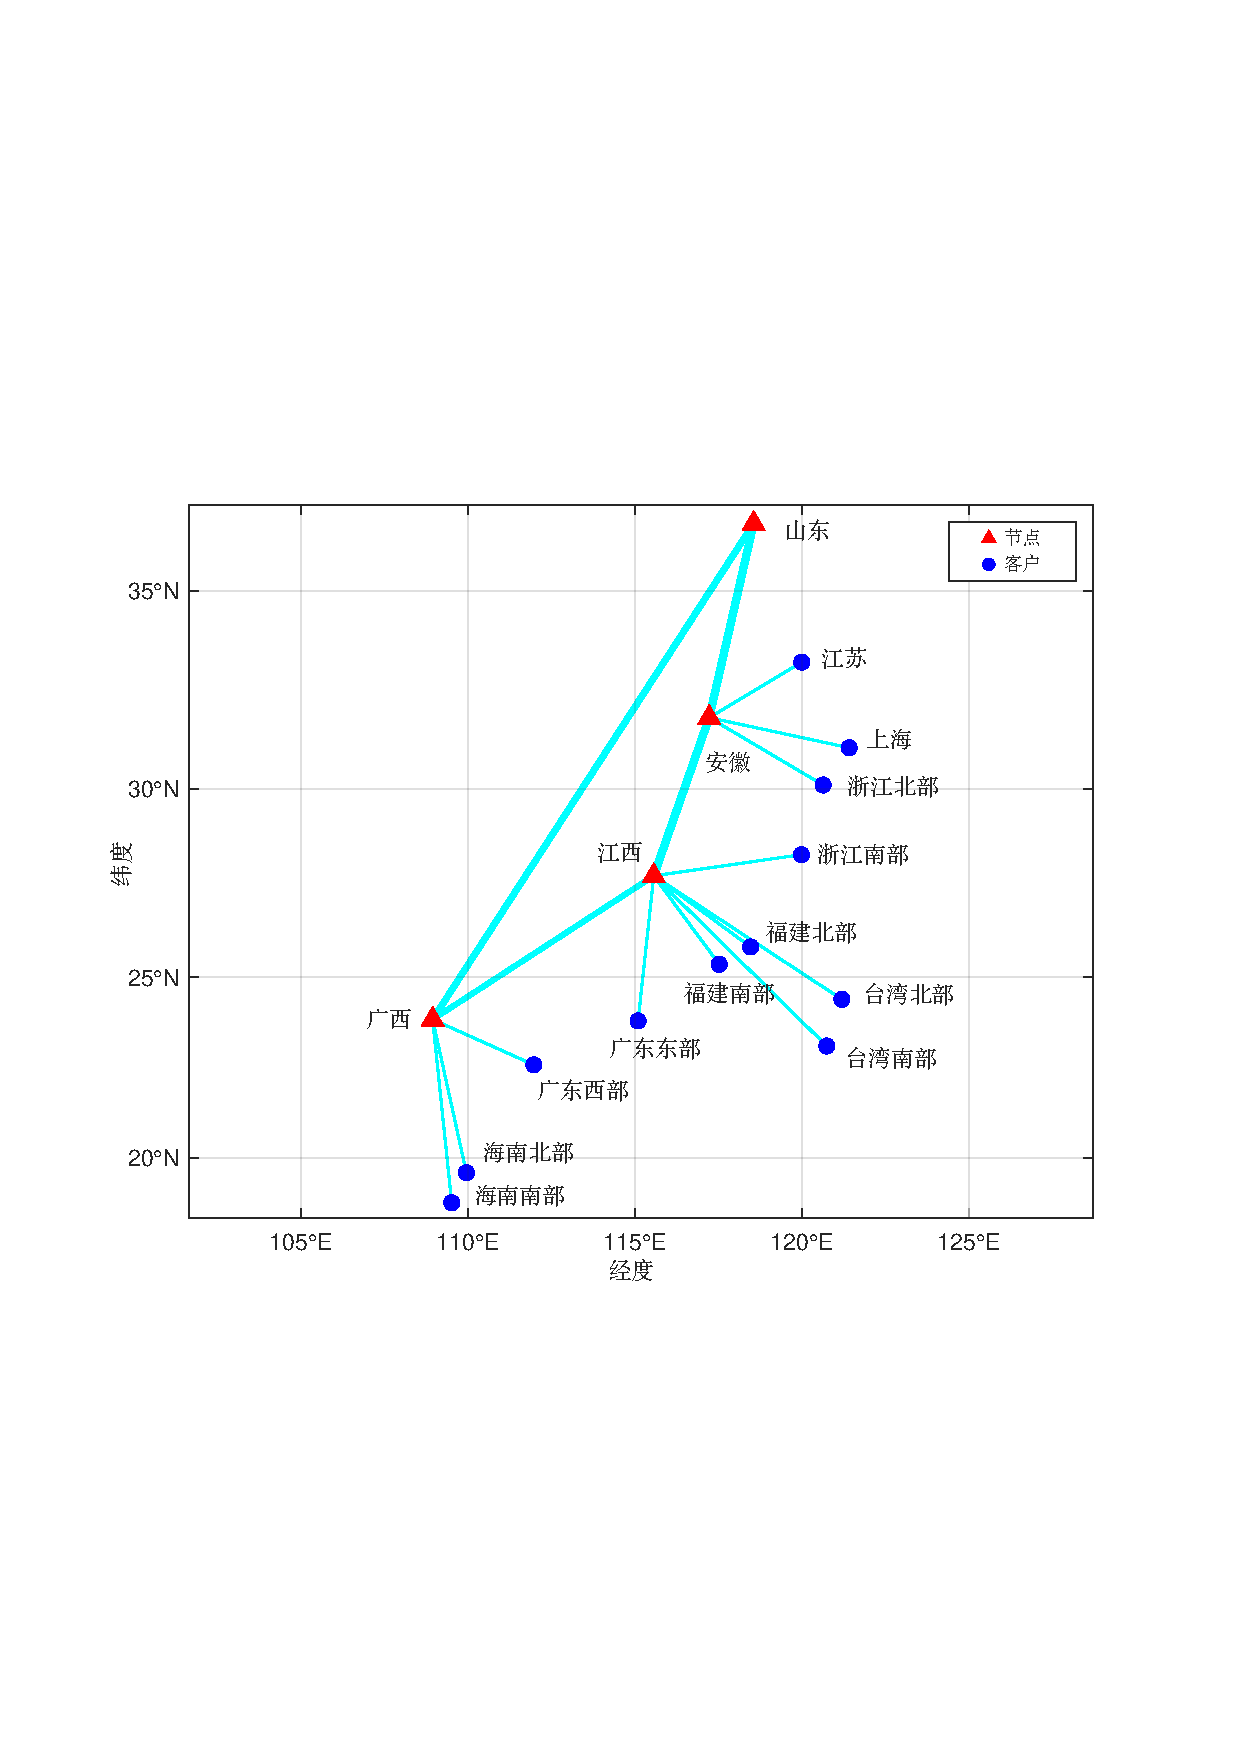
\includegraphics[height=0.4\textheight]{figures/case_location.pdf}
    \caption{东南沿海地区物流节点选址方案\\ Fig~\ref{fig:case_location}~ Southeast coastal region logistics node locating plan}
    \label{fig:case_location}
\end{figure}

图\ref{fig:case_location}中每个点均为客户点和候选点,
蓝色的圆点表示最终选址方案中不在该位置建设节点,
因此该点只有客户。
红色的三角形表示在该位置建设节点,
该点同时拥有节点和客户。
蓝绿色线条表示客户和其常用节点的指派关系,
若该线条连接一个客户和一个节点,
表示该客户将该节点设为常用节点,
若该线条连接两个节点,
表示两个节点同时作为某个客户的不同等级的实体节点。
并且两个节点之间的联系越强,
节点之间的线条越粗。

\begin{figure}[!b] %这里使用的是强制位置,除非真的放不下,不然就是写在哪里图就放在哪里,不会乱动
	\centering  %图片全局居中
	\vspace{-0.35cm} %设置与上面正文的距离
	\subfigtopskip=2pt %设置子图与上面正文或别的内容的距离
	\subfigbottomskip=2pt %设置第二行子图与第一行子图的距离,即下面的头与上面的脚的距离
	\subfigcapskip=-5pt %设置子图与子标题之间的距离
	\subfigure[常用节点]{
		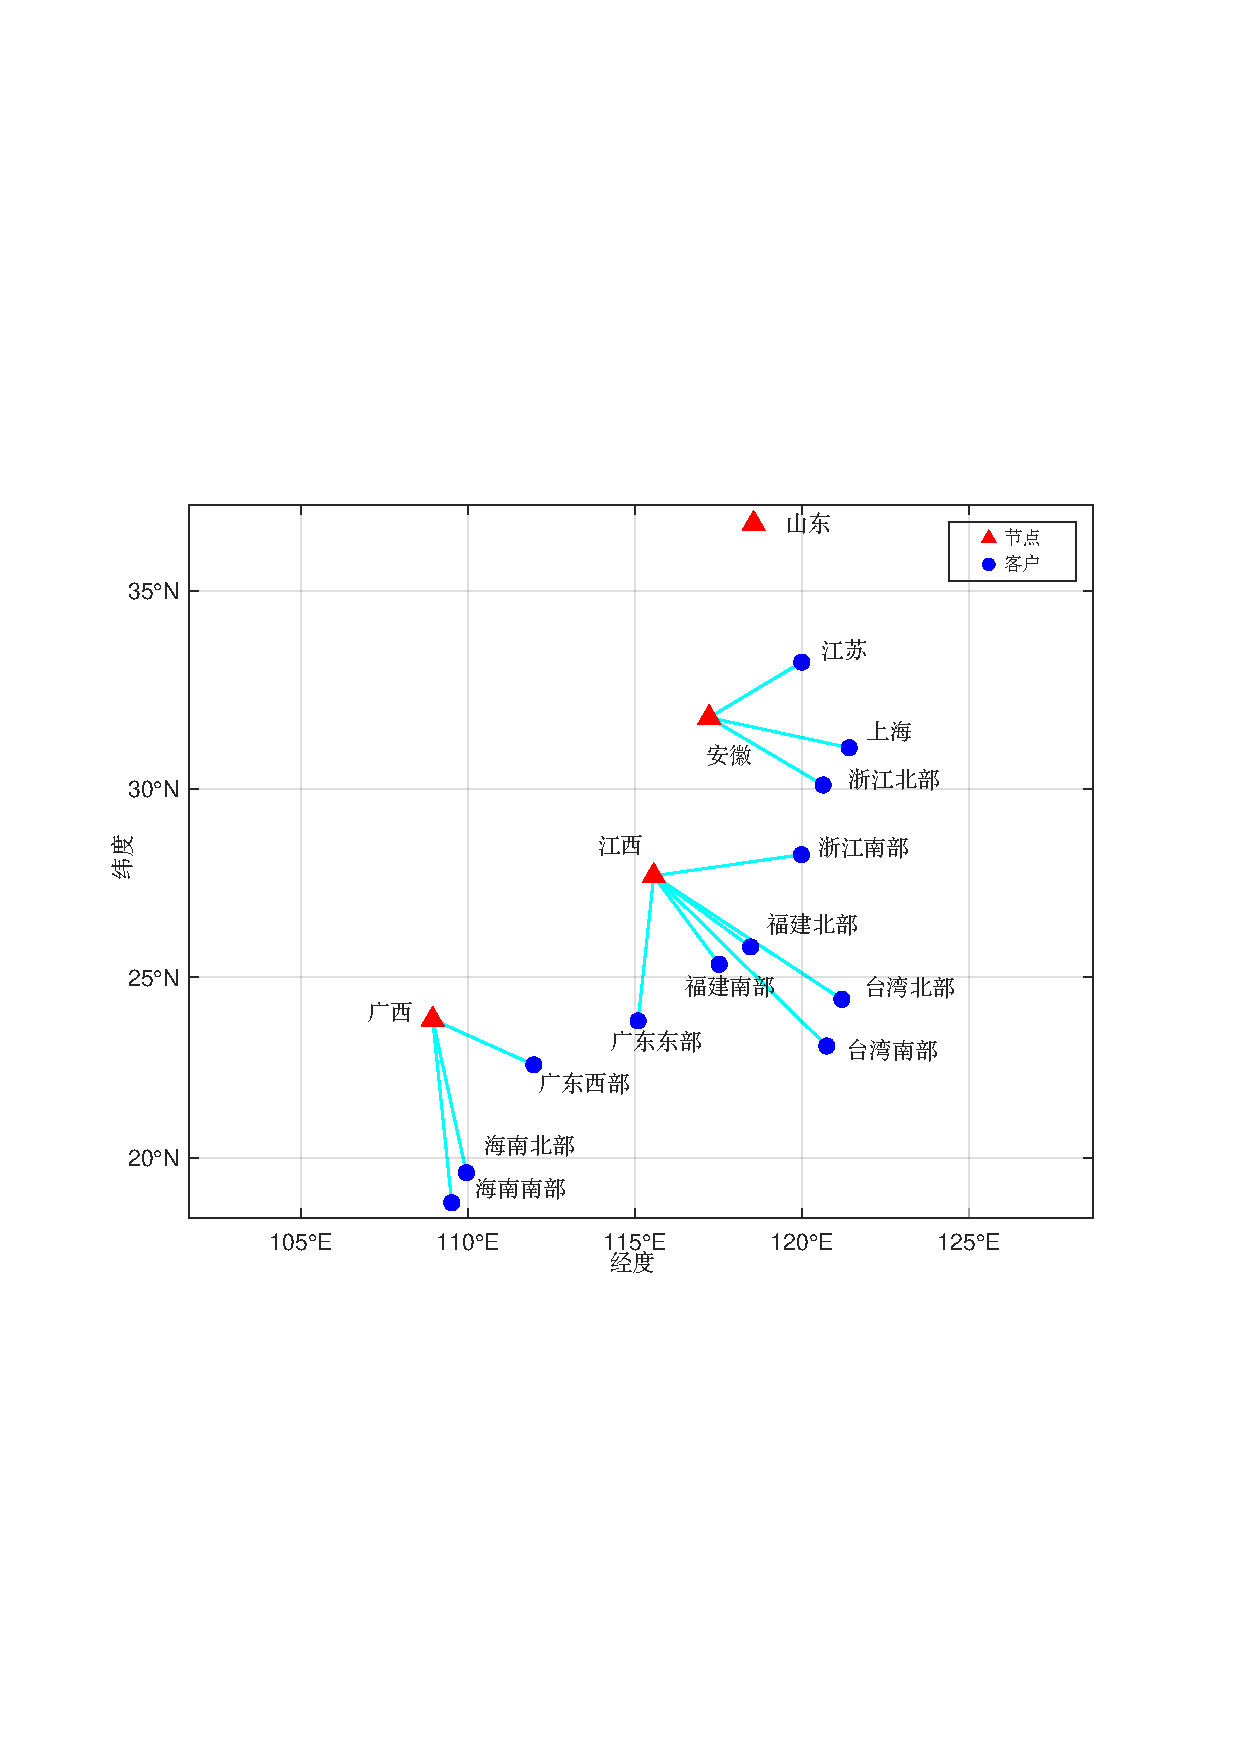
\includegraphics[width=0.47\linewidth]{figures/case_r_1.pdf}}
	\quad %默认情况下两个子图之间空的较少,使用这个命令加大宽度
	\subfigure[一级备用]{
		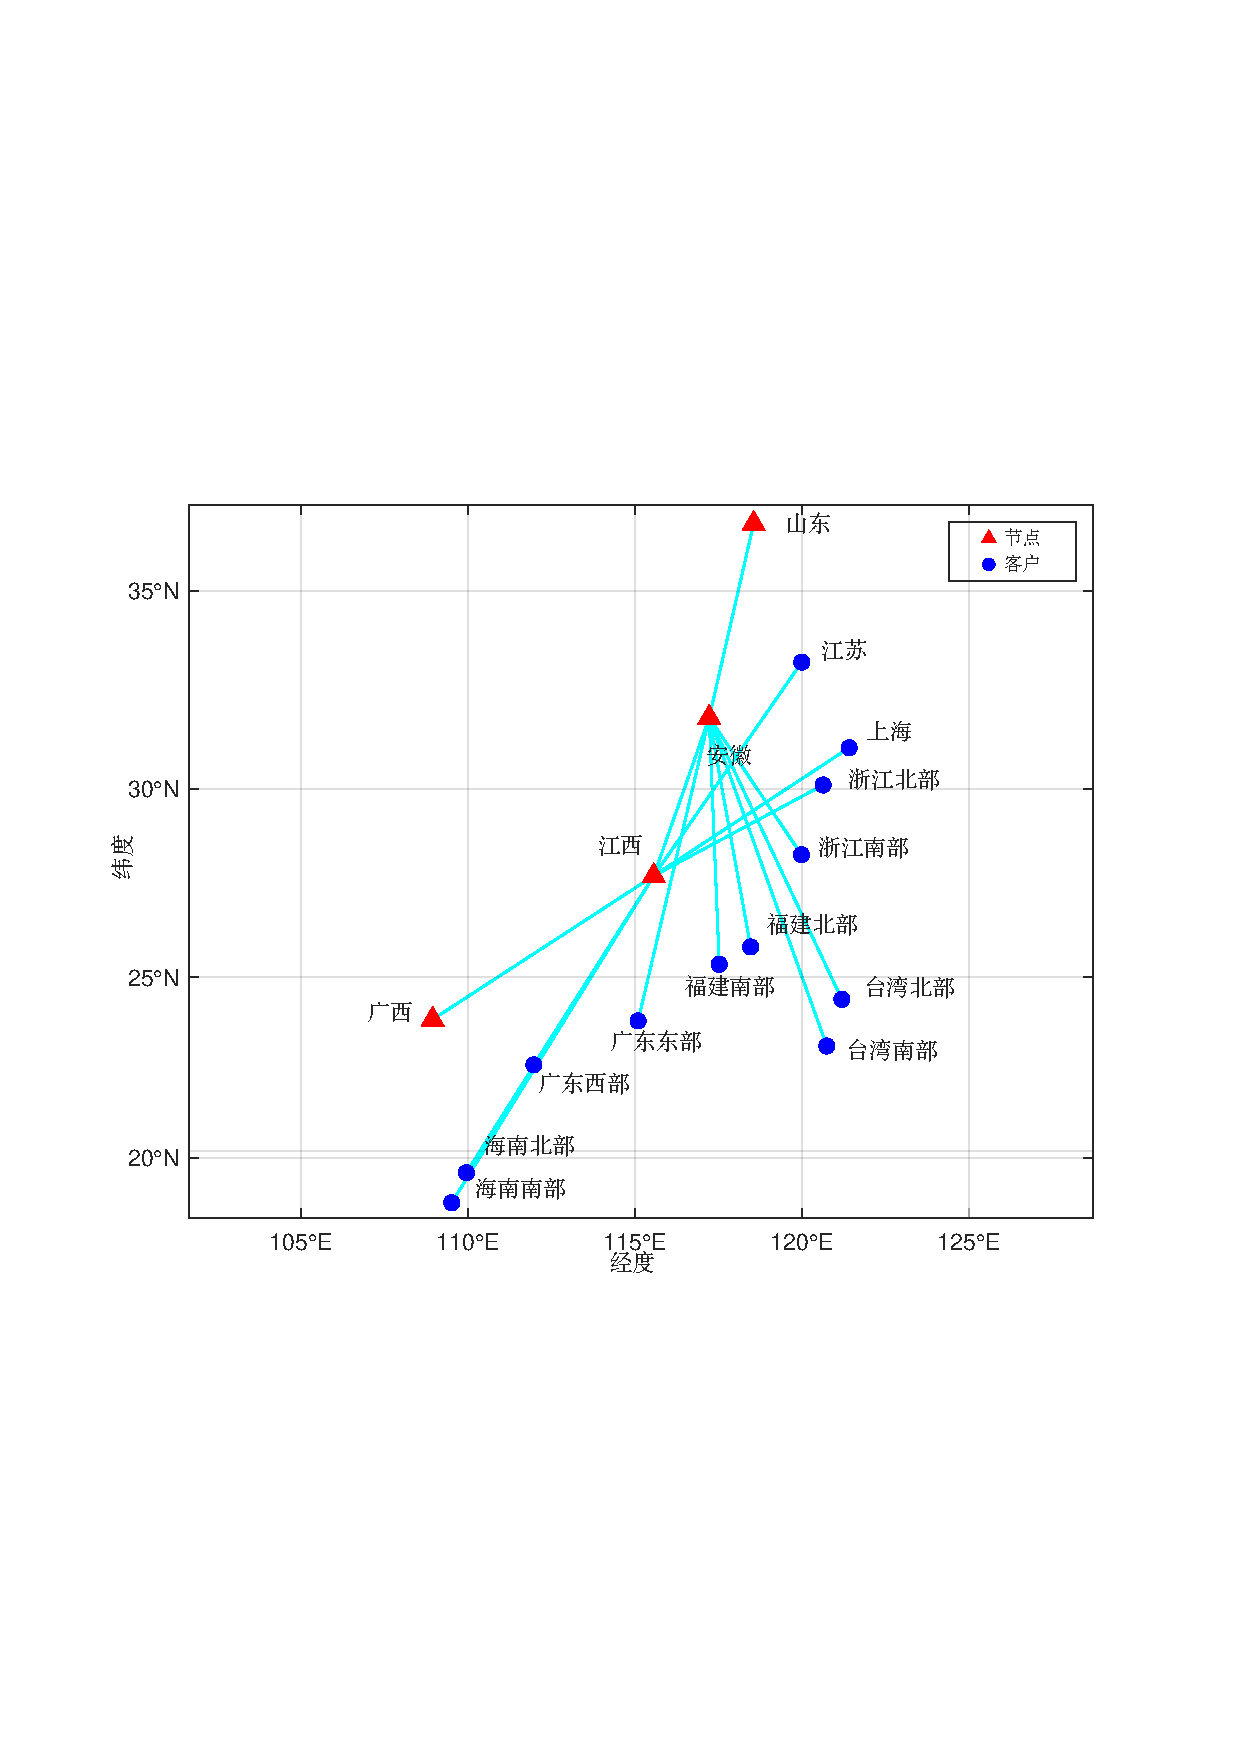
\includegraphics[width=0.47\linewidth]{figures/case_r_2.pdf}}
	  %这里是空了一行,能够实现强制将四张图分成两行两列显示,而不是放不下图了再换行,使用\\也行。
	\subfigure[二级备用]{
		% \includegraphics[width=0.47\linewidth]{figures/result_mp_rho0.2.eps}}
		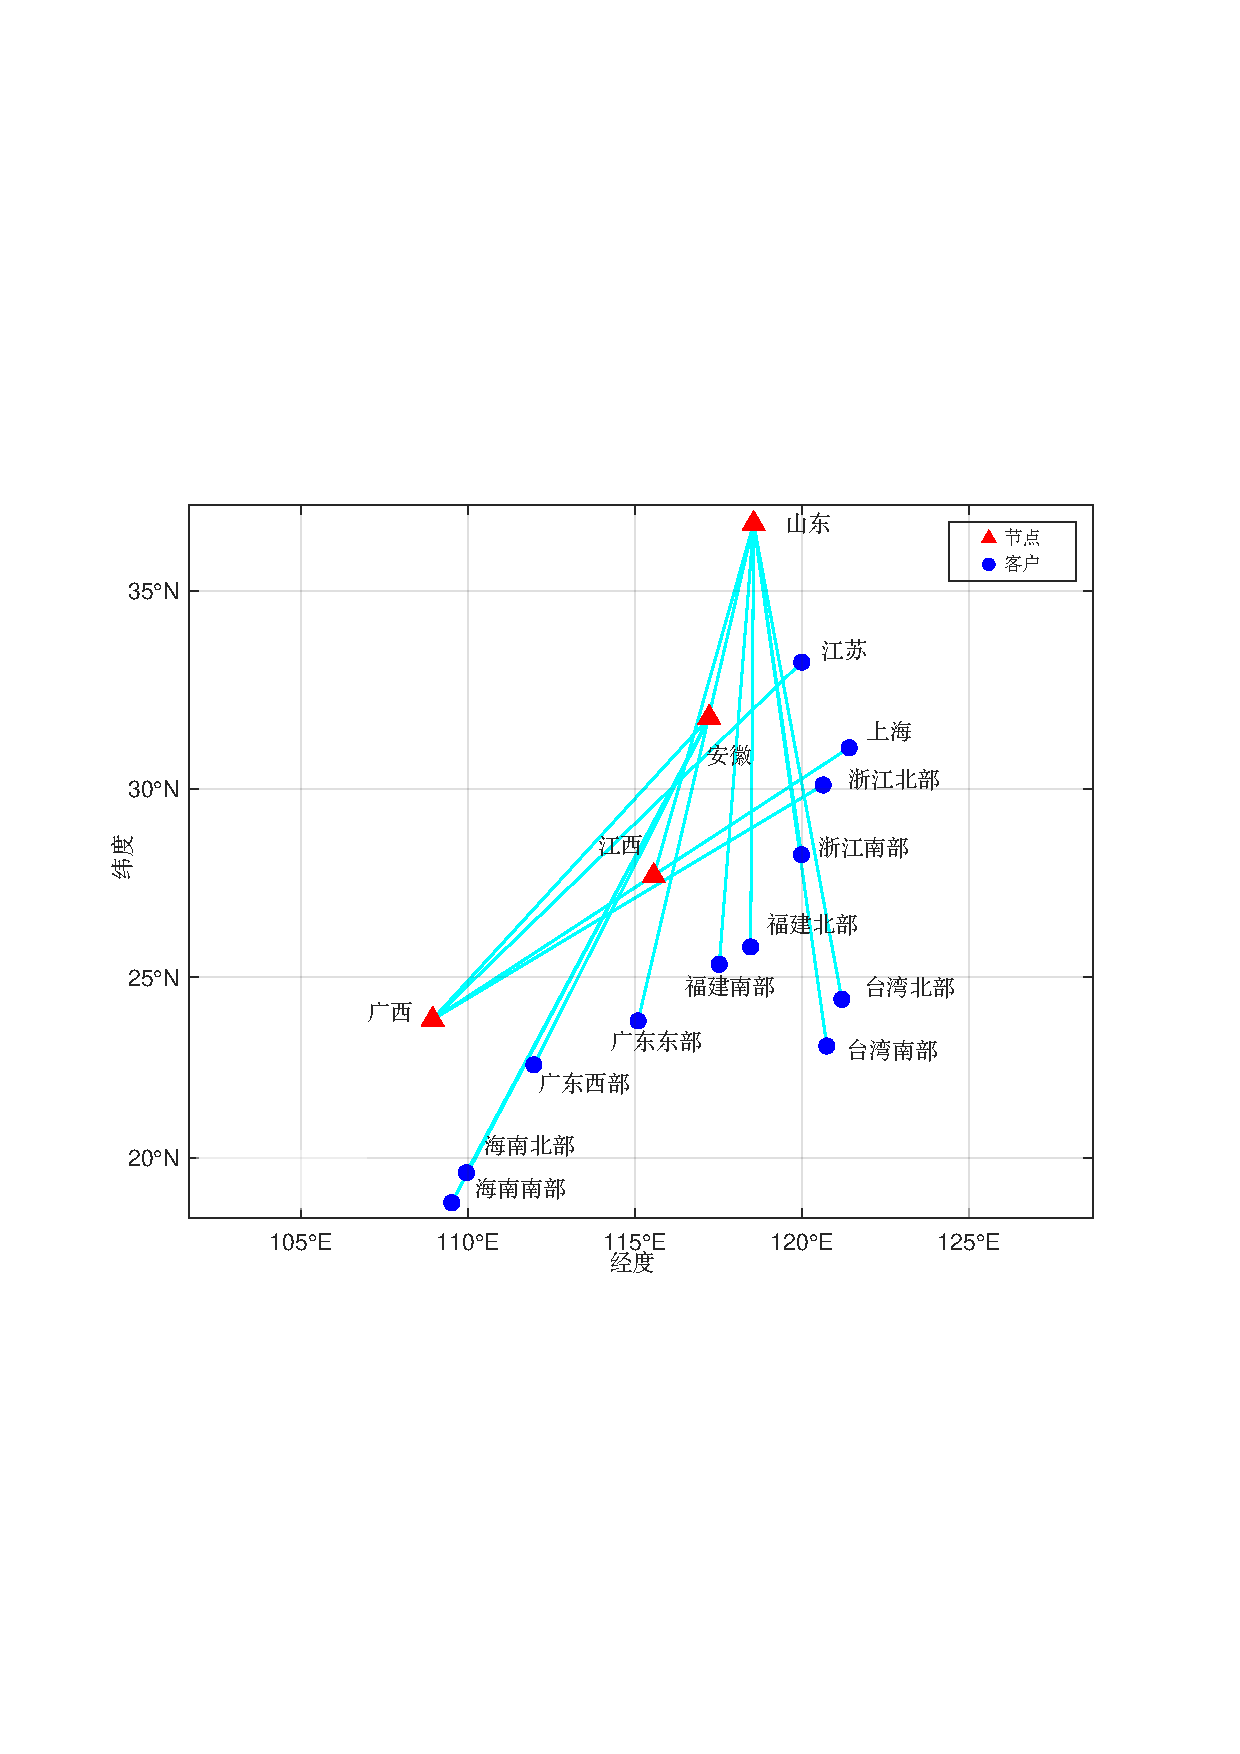
\includegraphics[width=0.47\linewidth]{figures/case_r_3.pdf}}
	\quad
	\subfigure[三级备用]{
		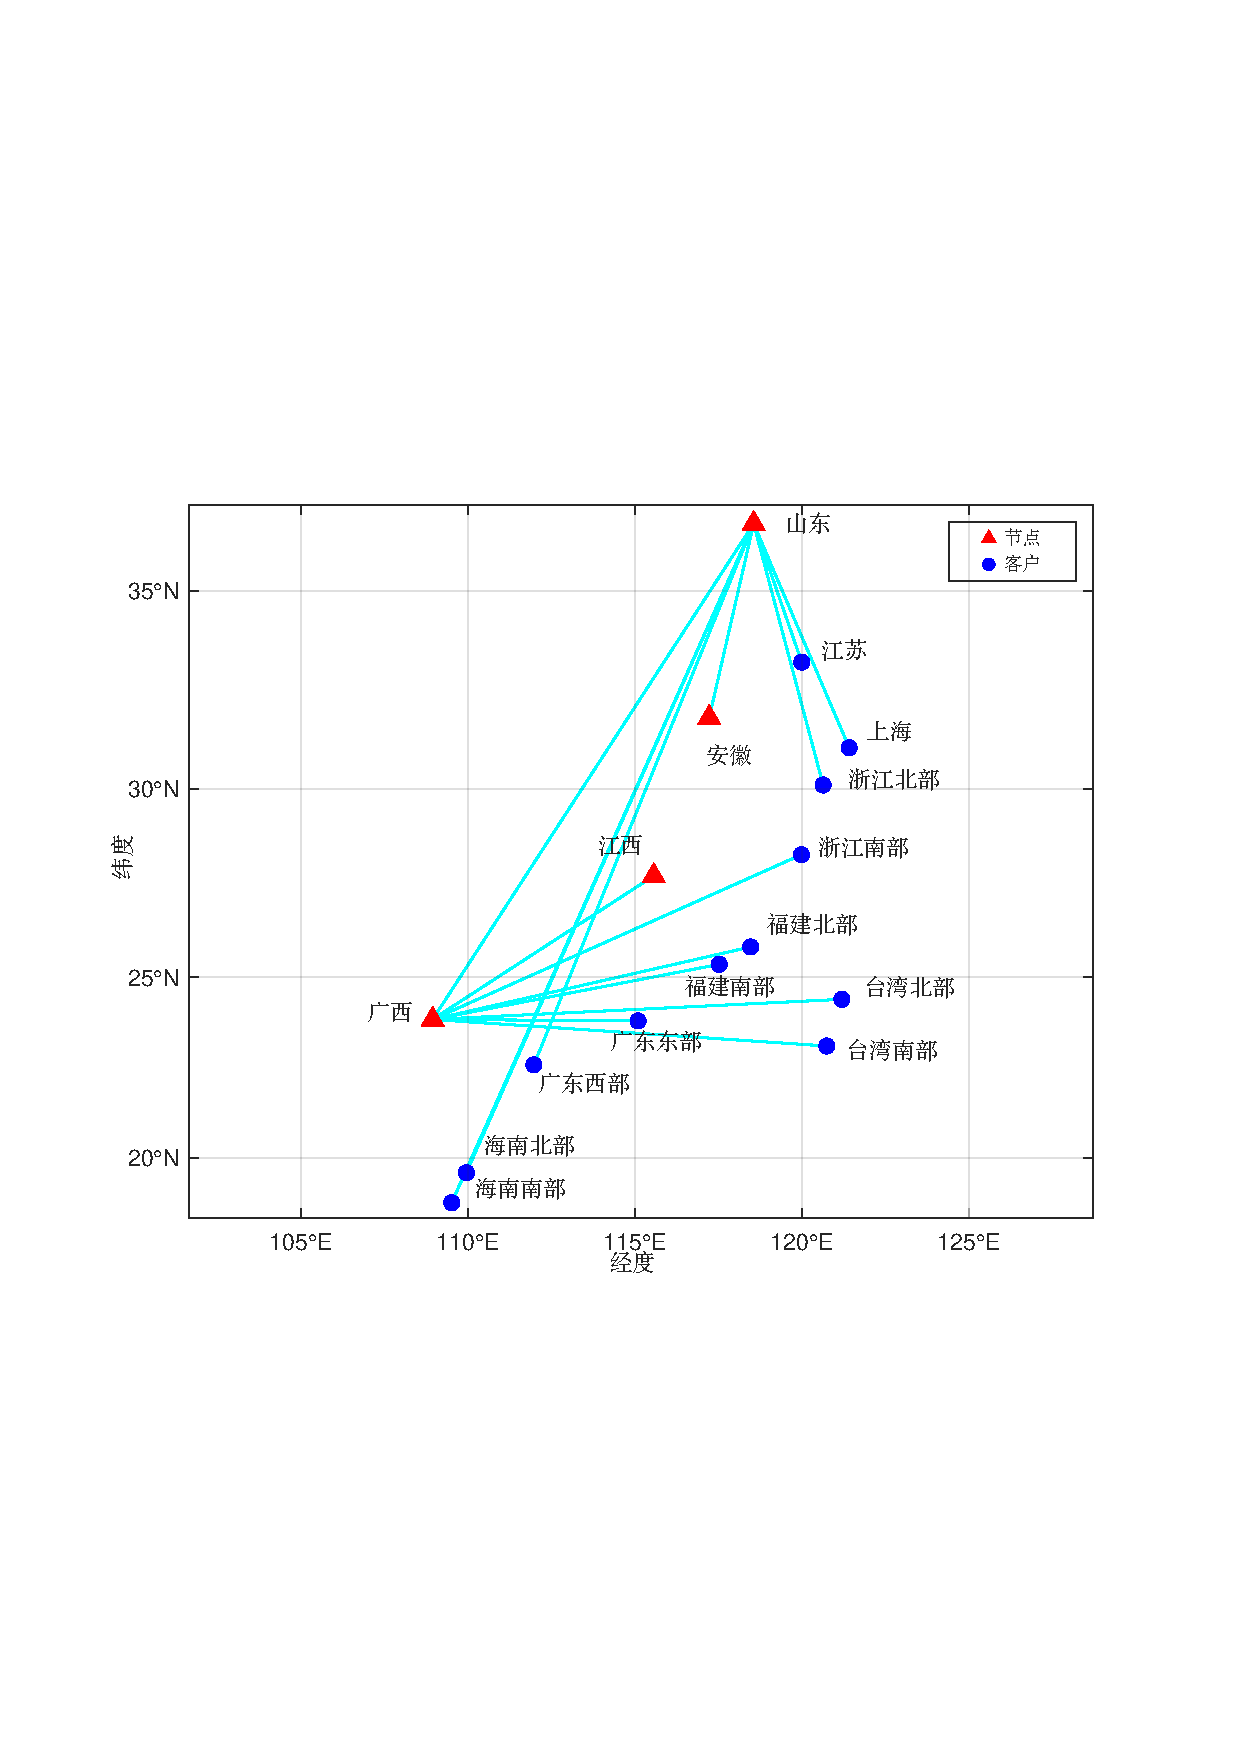
\includegraphics[width=0.47\linewidth]{figures/case_r_4.pdf}}
	\caption{客户的常用节点和备用节点\\Fig~\ref{fig:case_backup}~ Primary and backup nodes for customers}
	\label{fig:case_backup}
	\vspace{-0.35cm} %设置与上面正文的距离
\end{figure}


从图\ref{fig:case_location}中可观察到,在案例网络中,节点最佳选址一般都位于内陆地区,
这些地区受台风影响较小,
因此相关节点的失效概率更低,
在这些地区建设节点可以规避风险、降低因节点失效产生的惩罚成本。
此外,这些地区建设节点的固定成本较低,
因此模型更倾向于选择这些地区以权衡固定成本和期望运输成本。
从地理位置来看,
物流节点建设位置南北分布相对较为均匀,
且一般情况下一个节点为多个客户提供服务。
但注意到节点14(山东)仅作为客户14(山东)的常用设施,
产生这样的特殊情况的原因是在该网络中,
节点14处于相对较为偏远的地理位置,
并且其需求量相对较高而建设成本将对较低,
如不在此处建设节点,则期望运输成本的增量变化可能会大于在点14建设节点的成本。
此外,节点14不仅是客户14的常用节点,
还是其他客户的备用节点。
节点14凭借相对较低的建设成本和较低的失效概率
提高了网络整体的可靠性。
图\ref{fig:case_backup}展示了每个客户的常用节点和不同等级的备用节点方案。
在本案例中,
通常每个客户选择距离自己相对较近的节点作为自己的常用节点,
选择较近的节点作为常用节点可降低大多数情况下的运输成本。
当客户的常用节点失效时,
客户前往一级备用节点。
在本案例中,由节点13(江西)和节点15(安徽)作为所有客户的一级备用节点,
每个节点分别服务8个客户。
而二级备用节点分布较为广泛,
四个节点同时成为不同客户的二级节点。
对于客户的三级备用节点安排,
与一级备用节点截然不同,
位于较为偏僻的节点11(广西)和14(山东)。
特别地,
客户点12(江苏)使用节点15(安徽)作为常用节点,
使用节点13(江西)作为一级备用节点,
使用节点11(广西)作为二级备用节点,
而距离相对较近的节点14(山东)则成为了三级备用节点。
这表明在可靠选址模型中,
并非距离越近越能成为使用频率较高的备用节点。
本案例的结果恰好建设了四个节点,
节点13(江西)和节点15(安徽),
作为整个网络中超过一半数量的客户的常用节点
以及全部客户的备用节点,
这两个节点的可靠性直接决定整个网络的可靠性和系统的总成本。

上述节点选址方案呈现出以下特征:
(1)如果某个候选点的失效概率相对较低并且建设成本较小,
更适合在此处建设节点。
(2)在沿海地区构建物流网络时,
腹地更适合建设物流节点。
(3)选择距离相对较近的节点作为客户常用节点的同时,
也应当综合考虑节点的失效概率。
(4)地理位置相对居中的节点更容易作为客户的的备用节点,
当这些节点失效后,客户才会去往更偏远的节点。

\section{参数灵敏度分析}
\label{sec:灵敏度}

本节将分析模型参数取值的变化对结果的影响,
考察选址方案、成本构成随参数变动而变动的趋势,
并提出管理意见。
主要研究了参数设置中$R$,节点失效概率,运价波动的影响。
本小节并未考虑惩罚价格$\pi$的影响,
在相对可靠的模型中,
惩罚价格产生的期望惩罚成本在总成本中所占的比重非常小(参见$R$变动的情况),
因此并不能显著影响选址决策。

\subsection{参数\texorpdfstring{$R$}{R}灵敏度分析}

参数$R$控制每个客户拥有的常用节点和备用节点的数量,
为探究客户可拥有的节点的数量对选址结果、成本变动和成本构成的影响,
选取了$R$大于等于2小于且小于等于6的整数值。
表\ref{table:sens_R}展示了$R$不同取值对选址结果和成本的影响。

在本案例中,
选址方案的鲁棒性较强,
参数$R$的取值并未对选址方案造成影响,
但显著影响了系统的期望运输成本。
在本小节中当前和接下来的内容中,
系统的期望运输成本可拆分成惩罚成本和惩罚成本之外的运输成本。
当$R$取值较小时,
系统的总成本很高的直接原因是惩罚成本较高,
根本原因是客户的备用节点数量太少,
其拥有的所有节点全部失效的概率较高,
因此产生了较高的惩罚成本。
当$R$取值相对较大时,
惩罚成本占比较低几乎可以忽略不计,
此时认为系统处于相对可靠的状态。


\begin{table}[htbp]
\renewcommand{\arraystretch}{0.9}
\setlength{\abovecaptionskip}{-0.05cm} %调整图片caption与正文之间的间距,table同理。可自己调整。
\setlength{\belowcaptionskip}{-0.2cm} 
\centering
\renewcommand\arraystretch{1}
\caption{不同参数$R$取值的选址结果
		\\Table~\ref{table:sens_R}~Results for different $R$}
	\small{
		\begin{tabular}{cccccr}
			\toprule %[2pt]设置线宽 
			\multirow{2}[0]{*}{$R$} & \multirow{2}[0]{*}{选址方案} & \multirow{2}[0]{*}{总成本} & \multirow{2}[0]{*}{固定成本} & \multicolumn{2}{c}{期望运输成本} \\
			\cmidrule{5-6}
			&       &       &       & 运输成本  & \multicolumn{1}{c}{惩罚成本} \\
			\midrule
			2     & 11,13,14,15 & 11643707.32 & 3124950.00 & 3749804.67 & 4768952.65  \\
			3     & 11,13,14,15 & 7299791.68 & 3124950.00 & 4048818.54 & 126023.14  \\
			4     & 11,13,14,15 & 7180146.87 & 3124950.00 & 4052103.67 & 3093.20  \\
			5     & 11,13,14,15 & 7176847.65 & 3124950.00 & 4051767.43 & 130.22  \\
			6     & 11,13,14,15 & 7176847.65 & 3124950.00 & 4051767.43 & 130.22  \\
			\bottomrule
		\end{tabular}%
	}
\label{table:sens_R}
\end{table}%

  
系统总成本随参数$R$的增加而快速下降,
然后下降逐渐缓慢。
最后,即便参数$R$增加,
系统的惩罚成本和总成本也不再下降。
这表明单纯依靠增加客户的备用节点的数量
以提升网络的可靠性是有边界限制的。
超过此数量边界后,
即便再增加客户的备用节点数量,
也不能降低系统的成本。
在本案例研究中,
客户拥有一个常用节点和三个备用节点是相对合理的,
既使得系统总成本相对较低,
又获得了一个可靠的网络。
对于整个问题来说,
$R$等于2时该问题退化至经典UFL问题,
系统的总成本非常高,
但只要为每个客户安排一个备用节点,
系统总成本将降低37.3\%,
这充分体现了备用节点对于降低系统成本、
提升网络可靠性发挥的重要作用。


\subsection{节点失效概率灵敏度分析}
节点的失效概率是影响物流节点可靠选址模型结果的一个重要因素,
本文定义了函数$q_j' = \beta \sqrt{2q_j - q_j^2},\forall j \in J $
用于缩放节点的失效概率,
其中,参数$\beta (0 \le \beta \le \min \{ 1/q'_j \})$
为缩放系数,
用于放大或缩小节点的失效概率,
$\beta$取值越大,则节点失效概率越高。
默认参数$R=5$,
使用上述函数更新每个节点的失效概率,
令参数$\beta$分别取0.1至2.0间隔为0.1的小数。
系统选址方案、成本变动和成本构成随节点失效概率变化而变化的结果
如表\ref{table:sens_prob}所示。

\begin{table}[htbp]
    \setlength{\abovecaptionskip}{-0.05cm} %调整图片caption与正文之间的间距,table同理。可自己调整。
    \setlength{\belowcaptionskip}{-0.2cm} 
    \centering
    \renewcommand\arraystretch{0.9}
    \caption{不同参数$\beta$取值的选址结果\\Table~\ref{table:sens_prob}~Results for different $\beta$}
    \small
    \begin{tabular}{cccrccr}
        \toprule %[2pt]设置线宽 
        \multicolumn{1}{c}{\multirow{2}[0]{*}{$\beta$}} & \multicolumn{1}{c}{\multirow{2}[0]{*}{平均失效概率}} & \multirow{2}[0]{*}{选址方案} & \multicolumn{1}{c}{\multirow{2}[0]{*}{总成本}} & \multicolumn{1}{c}{\multirow{2}[0]{*}{固定成本}} & \multicolumn{2}{c}{期望运输成本} \\
        \cmidrule{6-7}
        &       &       &       &       & \multicolumn{1}{c}{运输成本} & \multicolumn{1}{c}{惩罚成本} \\
        \midrule
        0.1   & 0.0280 & 11,13,14,15 & 7090419.90 & 3124950.00 & 3965415.51  & 54.39  \\
        0.2   & 0.0561 & 11,13,14,15 & 7345247.85 & 3124950.00 & 4219427.67  & 870.18  \\
        0.3   & 0.0841 & 11,13,14,15 & 7617992.88 & 3124950.00 & 4488637.61  & 4405.27  \\
        0.4   & 0.1121 & 11,13,14,15 & 7913784.74 & 3124950.00 & 4774911.92  & 13922.82  \\
        0.5   & 0.1401 & 11,13,14,15 & 8239058.47 & 3124950.00 & 5080117.21  & 33991.26  \\
        0.6   & 0.1682 & 11,13,14,15 & 8601554.35 & 3124950.00 & 5406120.08  & 70484.27  \\
        0.7   & 0.1962 & 11,13,14,15 & 9010317.95 & 3124950.00 & 5754787.14  & 130580.81  \\
        0.8   & 0.2242 & 11,13,14,15 & 9471654.72 & 3124950.00 & 6123939.63  & 222765.09  \\
        0.9   & 0.2522 & 11,12,13,14,15 & 9937270.28 & 4319380.00 & 5306396.32  & 311493.96  \\
        1.0   & 0.2803 & 11,12,13,14,15 & 10426426.71 & 4319380.00 & 5632280.73  & 474765.98  \\
        1.1   & 0.3083 & 11,12,13,14,15 & 10988921.36 & 4319380.00 & 5974436.49  & 695104.87  \\
        1.2   & 0.3363 & 11,12,13,14,15 & 11638030.42 & 4319380.00 & 6334175.69  & 984474.73  \\
        1.3   & 0.3643 & 11,12,13,14,15 & 12387706.57 & 4319380.00 & 6712347.46  & 1355979.11  \\
        1.4   & 0.3924 & 11,12,13,14,15 & 13253041.92 & 4319380.00 & 7109800.94  & 1823860.98  \\
        1.5   & 0.4204 & 10,11,13,14,15 & 14240588.43 & 4806730.00 & 7608669.63  & 1825188.80  \\
        1.6   & 0.4484 & 10,11,13,14,15 & 15210335.33 & 4806730.00 & 8040828.58  & 2362776.75  \\
        1.7   & 0.4765 & 9,10,13,14,15 & 16038348.93 & 5629860.00 & 8100631.15  & 2307857.78  \\
        1.8   & 0.5045 & 9,10,13,14,15 & 16924979.02 & 5629860.00 & 8394415.26  & 2900703.76  \\
        1.9   & 0.5325 & 9,10,13,14,15 & 17931541.49 & 5629860.00 & 8700643.02  & 3601038.47  \\
        2.0   & 0.5605 & 9,10,13,14,15 & 19070759.66 & 5629860.00 & 9019769.10  & 4421130.56  \\
        \bottomrule  
    \end{tabular}%
    \label{table:sens_prob}
\end{table}%

为方便理解不同$\beta$取值下失效概率的变化情况,
表\ref{table:sens_prob}给出了节点的平均失效概率,
随着$\beta$增加,
节点的平均失效概率从0.0280增加至0.5605。
随着节点的失效概率增加,
节点选址的数量由4个增加至5个,
其中节点13(江西)、14(山东)、15(安徽)出现在当前所有的选址结果中,
表明在节点的失效概率存在扰动的情况下,
在这些位置建设节点的选址结果具有鲁棒性,
可以应对不同的大小节点失效概率并保持选址结果稳定。
随着$\beta$增加,
系统的各项成本随$\beta$值的增加而增加。
对于惩罚成本,
节点失效概率增加,
导致客户更容易面对所有备用节点全部失效的情况,
此时惩罚成本随之增加。
同理,节点失效概率增加,
导致客户前往其他节点的概率增加,
即运输成本随之上升。
为了降低期望运输成本,
系统不得不建设更多的节点阻止更多的期望运输成本产生,
但建设更多的节点产生了更多的固定成本。

\begin{figure}[!hbt] % use float package if you want it here
	%\setlength{\abovecaptionskip}{-0.2cm} %调整图片caption与正文之间的间距,table同理。可自己调整。
	\setlength{\belowcaptionskip}{-0.5cm} 
	  \centering
	  \includegraphics[width = 0.9 \textwidth]
	  {figures/sens_tradeoff.pdf}
	  \caption{成本随$\beta$变动的权衡曲线\\
	  Fig~\ref{fig:sens_tradeoff}~ Trade-off curves for the variation of each cost with $\beta$}
	  \label{fig:sens_tradeoff}
\end{figure}

图\ref{fig:sens_tradeoff}直观展示了四项成本的权衡曲线,
随着参数$\beta$的增加,
成本变化的权衡曲线可分成三个阶段。
第一阶段($0.1\le \beta \le 0.8$),
节点的失效概率相对较小,
因此惩罚成本在总成本中的占比较小,
并不能影响选址决策。
但是随着节点的失效概率增加,
每个客户可能会访问更多的备用节点,
因此运输成本快速增长。
在$\beta=0.1$时,
运输成本和固定成本的大小是接近的,
但在$\beta=0.8$时,
运输成本显著高于固定成本。
此时,优化结果第一次调整进入第二阶段($0.9 \le \beta \le 1.4$),
增加建设了一个节点以降低运输成本。
在$\beta=0.9$时,
可看到运输成本显著降低、
固定成本显著上升的变化趋势。
然后,结果重复第一阶段的趋势,
维持选址结果不变,
惩罚成本、运输成本增加。
进入第三阶段($1.5 \le \beta \le 2.0$),
惩罚成本增加的速率明显增加、占总成本比重增加,
惩罚成本可以显著影响选址结果。
在第三阶段共发生了两次节点数量不变,
但位置发生变化的调整(节点10替换节点12,节点9替换11)。
这两次节点替换调整都是使用了失效概率较小的节点替换了失效概率较大的节点,
这样的调整虽然增加了建设节点的固定成本,
但一定程度上缓和了运输成本和惩罚成本增长的趋势。

上述分析表明东南沿海地区物流节点选址案例的
选址方案可以承受节点失效概率的变动,
但这种承受能力是有限度的。
当节点失效概率普遍较小时($\le$22\%),
选址方案几乎不会变动,
当节点的失效概率相对较大时($\ge 22\%$且$\le 39\%$),
降低总成本的办法是增加节点建设的数量。
当节点失效概率普遍非常大时($\ge 39\%$且$\le 56\%$),
降低总成本的方法是用失效概率较小的候选节点替换失效概率比较大的节点。


\subsection{运价灵敏度分析}
除了上述节点的失效概率会对选址结果产生影响以外,
运价的变动同样会影响节点的选址。
在本模型中,运输成本等于运价乘以需求,
因此,运价系数的变化同样可以看作是客户需求的变化。
下面以运价变化为例,
分析其对选址结果的影响。

为了探究运价变动对选址结果的影响,
分别调整运价系数至0.5至2.0间隔为0.1的16个值,
表\ref{table:sens_price}展示了不同价格系数下的最优节点选址方案。
随着运价系数增加,
节点的选址数量也从3个逐个增加至6个。
在运价较低时,
只需三个节点就可以胜任整个网络的任务,
此时的惩罚成本相对较高,
但在总成本中的比重可忽略不计,
每个客户拥有一个常用节点和两个备用节点,
系统仍然保持了可靠性。
在本案例的默认情况下,
运价系数等于1.1,
表\ref{table:sens_price}中运价系数在0.7至1.6的范围内变动时,
选址方案不变。
这表明案例的选址方案可在大幅度的运价波动保持其方案最优性。
运价系数线性增加,
总成本也相应增加,
总成本主要由固定成本和运输成本构成,
惩罚成本可忽略不计。
虽然总成本具有上升的趋势,
但固定成本和运输成本的占比在不断变化。
图\ref{fig:sens_price}展示了固定成本、运输成本和惩罚成本的权衡,
以及总成本的变化趋势。



\begin{table}[htbp]
    \setlength{\abovecaptionskip}{-0.05cm} %调整图片caption与正文之间的间距,table同理。可自己调整。
    \setlength{\belowcaptionskip}{-0.2cm} 
    \centering
    \renewcommand\arraystretch{0.9}
    \caption{不同运价系数取值的选址结果。
    \\Table~\ref{table:sens_price}~Results for different shipping rates.}
    \small{
        \begin{tabular}{cccccc}
            \toprule %[2pt]设置线宽 
            \multirow{2}[0]{*}{运价系数} & \multirow{2}[0]{*}{选址方案} & \multirow{2}[0]{*}{总成本} & \multirow{2}[0]{*}{固定成本} & \multicolumn{2}{c}{期望运输成本} \\
            \cmidrule{5-6}
                &       &       &       & 运输成本  & 惩罚成本 \\
            \midrule
            0.5   &  11,13,15 & 4719194.69 & 2187680.00 & 2525595.46  & 5919.23  \\
            0.6   &  11,13,15 & 5224313.78 & 2187680.00 & 3030714.55  & 5919.23  \\
            0.7   &  11,13,14,15 & 5703477.68 & 3124950.00 & 2578397.46  & 130.22  \\
            0.8   &  11,13,14,15 & 6071820.17 & 3124950.00 & 2946739.95  & 130.22  \\
            0.9   &  11,13,14,15 & 6440162.67 & 3124950.00 & 3315082.45  & 130.22  \\
            1.0   &  11,13,14,15 & 6808505.16 & 3124950.00 & 3683424.94  & 130.22  \\
            1.1   &  11,13,14,15 & 7176847.65 & 3124950.00 & 4051767.43  & 130.22  \\
            1.2   &  11,13,14,15 & 7545190.15 & 3124950.00 & 4420109.93  & 130.22  \\
            1.3   &  11,13,14,15 & 7913532.64 & 3124950.00 & 4788452.42  & 130.22  \\
            1.4   &  11,13,14,15 & 8281875.13 & 3124950.00 & 5156794.91  & 130.22  \\
            1.5   &  11,13,14,15 & 8650217.63 & 3124950.00 & 5525137.41  & 130.22  \\
            1.6   &  11,13,14,15 & 9018560.12 & 3124950.00 & 5893479.90  & 130.22  \\
            1.7   &  11,12,13,14,15 & 9360502.47 & 4319380.00 & 5040974.92  & 147.55  \\
            1.8   &  2,11,12,13,14,15 & 9629435.45 & 5436860.00 & 4192288.53  & 286.92  \\
            1.9   &  2,11,12,13,14,15 & 9862340.37 & 5436860.00 & 4425193.45  & 286.92  \\
            2.0   &  2,11,12,13,14,15 & 10095245.29 & 5436860.00 & 4658098.37  & 286.92  \\
            \bottomrule  
        \end{tabular}%
    }
    \label{table:sens_price}
\end{table}%

随着运输价格的增长,
总成本近似线性增加,
惩罚成本几乎可忽略不计,
因此最优选址方案和成本变化完全由系统的固定成本和运输成本决定。
图\ref{fig:sens_price}展示了固定成本和运输成本的权衡,
当运输成本上升至一定程度时,
系统往往会增加一个节点以降低系统的运输成本。
因此,固定成本曲线和运输成本曲线呈现互相交错的趋势。
虽然在此价格系数变化范围内,
系统的总成本是近似线性增加的,
但可以预见的是,
随着价格系数的不断增长,
建设的节点的数量也将随着增加,
最终最优的选址方案是在每个候选点建设一个设施,
此时系统的固定成本不变,
总成本是价格系数的线性函数。
由于每个客户的备用节点数量充足,
惩罚成本同样不会占比过高。

\begin{figure}[!h] % use float package if you want it here
	%\setlength{\abovecaptionskip}{-0.2cm} %调整图片caption与正文之间的间距,table同理。可自己调整。
	\setlength{\belowcaptionskip}{-0.5cm} 
	  \centering
	  \includegraphics[width = 0.9 \textwidth]
	  {figures/sens_price.pdf}
	  \caption{成本随价格系数变动的权衡曲线\\
	  Fig~\ref{fig:sens_price}~ Trade-off curves for the variation of shipping rate}
	  \label{fig:sens_price}
\end{figure}

上述分析表明,
系统的选址方案受价格(需求)的影响较大,
运输价格或需求越高,
系统的总成本以及建设的节点数量随之增加。
并且在很大的范围内,
运价或需求的增加并不影响最优选址方案。
当运价或需求增加超过临界值,
系统会在原有建设节点基础上增加建设设施,
以缓解运输成本的增长。
这说明将该选址方案应用与现实中,
可应对长期的需求增长。
当需求增加超过一定幅度,
只需要增加建设一个新的节点即可,
为长期的决策实施提供了灵活方案。



\section{本章小结}
\label{sec:小结6}

本章研究了考虑台风灾害影响的东南沿海地区的物流节点可靠选址案例,
求解该案例并得到了东南沿海地区的物流可靠网络,
为每个客户指派了常用物流节点和备用节点方案。
案例选址结果展现了明显的空间特征:
将节点建设在沿海地区的腹地可在降低系统总成本的同时使系统更加可靠。
灵敏度分析结果表明,
为每个客户安排尽量多的备用节点所带来的边际收益是有限的,
为客户指派一个常用节点和三个备用节点是最合理的。
失效概率和客户的需求或运价的变动是影响系统选址的重要因素,
二者中任一增加都会使得系统的总成本增加,
系统的成本权衡曲线表明增加节点的数量是减缓总成本和运输成本增势的方法。
最后,虽然系统的总成本随参数变动而变动,
但选址的结果也展示出了较强的鲁棒性,
可抵御较大幅度的失效概率变动和运价或需求变动。


